\documentclass[]{article}
\usepackage[top=1in, bottom=1in, left=1.2in, right=1in, a4paper]{geometry}
 \ifx\pdftexversion\undefined
 \usepackage[dvips]{graphicx}
 \else
 
 \usepackage[pdftex]{graphicx}
 \DeclareGraphicsRule{*}{mps}{*}{}
 \fi
 %\usepackage{tabularx,colortbl}
\usepackage{url}
\usepackage{chapterbib}
\usepackage{hyperref}
\usepackage{tabularx}
%\usepackage{tikz}
%\usepackage{pgfplots}
%\usepgfplotslibrary{groupplots} 
%\usepackage{pgf, pgfarrows, pgfnodes}
\usepackage{lscape}
\usepackage{longtable}
\usepackage{float}
\usepackage{url}
\usepackage{multicol}
\usepackage{color}
\usepackage{float}

\begin{document}

%\begin{titlepage}
\begin{center}
\Large
\textbf{ \\ Cloud based IT Infra with Central Identity \\}
%
\normalsize
\textsf{ \\ Dept. of Computer Science and Engg. | \today  \\ }
%
\end{center}

\title{Cloud based IT Infra with Central Identity}
\author{Team r3b00+ }
%\maketitle

%\setcounter{page}{1}
%\pagenumbering{roman}

%\section*{Abstract}
%\begin{abstract}

\paragraph{Abstract \\}
\hspace{1.5cm} \\ \hspace{1.5cm} The main aim of Cloud based IT Infra with Central Identity is to develop central identity services for network based applications and web services using API calls. After implementing this we will get the services like single sign-on, role based user identity thus reduces the redundancy of data. We will mainly have 3 components Master Architecture, Slave Architecture and Cloud which connects both which will sufficiently provides the research and development requirements to our University. 
%\end{abstract}

%\vfill
%\begin{center}
%\today
%\end{center}


%\institute{Dept. of CSE, RGUKT - Nuzvid}

%\maketitle

\section*{Objectives under Development}

\begin{enumerate}

\item Central Identity for all applications and services.
\item Efficient utilization of existed Hardware.
%\item Facilitates high availability of all web-services (Like ONB, Examination, Course registration Helping hand website, SDCAC website and all departmental websites etc.)
%\item It will provide High computational power for research work of Faculty, research scholars and students.
%\item Get full recovery and  achieve 100\% Services up time.
\item Well structured \& controllable Network monitoring.
\item Dynamic user roles in Central Identity
\item Provide High computational power for research and development work.

\end{enumerate}


%\pagebreak

%\tableofcontents

%\pagebreak
%\setcounter{page}{1}
%\pagenumbering{arabic}
%\section{Objectives}
%
%\begin{enumerate}
%
%\item Central Identity for all applications and services.
%\item Efficient utilization of existed Hardware.
%%\item Facilitates high availability of all web-services (Like ONB, Examination, Course registration Helping hand website, SDCAC website and all departmental websites etc.)
%%\item It will provide High computational power for research work of Faculty, research scholars and students.
%%\item Get full recovery and  achieve 100\% Services up time.
%\item Well structured \& controllable Network monitoring.
%\item Dynamic user roles in Central Identity
%\item Provide High computational power for research and development work.
%
%\end{enumerate}
%
%\pagebreak

\section*{Present System}
\begin{itemize}
	\item Failed to maintain large user load services like ONB, Exam servers, etc.
	\item No proper Web Application Security \& Standards.
	\item No Central Identity, Storage \& High capacity hardware resource pool.
	\item Inadequate resource requirements for Research.
	\item Dedicated computer course labs like Matlab, VLSI, etc. 
\end{itemize}

\section*{Proposed System}
\begin{itemize}
	\item Cloud based hardware resource clustering.
	\item Central Identity to access Network Applicaitons using well designed API.
	\item Dynamic user roles in Central Identity for extended application support.
	\item New CPanel for Network Administration.
		\begin{itemize}
			\item Providing different user modes in OS, controlled remotely from CPanel.
			\item Providing Virtual Labs (machines) with desired resource capabilities.
			\item Providing a right to verify and approve user application requests.
		\end{itemize}
\end{itemize}

%\end{titlepage}

\pagebreak

\section*{Advantages}

\begin{itemize}
	\item Well structured \& controllable Network Administraion
	\item Efficient hardware utilization
	\item No registration for new Network based applications through Central Identity API
	\item Provding Virtual Machines with high hardware configuration for Researchers \& Developers
	\item Facilitates high availability of all web-services (Like ONB, Examination, Course registration Helping hand website, SDCAC website and all departmental websites etc.)
	\item It will provide High computational power for research work of Faculty, research scholars and students.
	\item Get full recovery and  achieve more than 99.99\% Services up time.
\end{itemize}


\section*{Requirements}
\begin{center}
\begin{itemize}
\item  10 Laptops % with 2 NICs
\begin{itemize}
	\item  8 GB RAM systems - 4 
	\item  4 GB RAM systems - 6 
	\begin{itemize}
		\item (We need to extend 4GB Ram to 8 GB RAM, We need to Extend One more NIC)
	\end{itemize}
	
\end{itemize}
 
\item Internet Facility 
\begin{itemize}
	\item 10 Static IP with full Internet access for lab with out proxy [ SF6 – 10.4.16.x ]
	\item 2 Proxy Accounts with Unlimited Downloading 
	\item Uninterrupted Internet Connectivity with 512KBPS+ Downloading Speed.
	\item Basically we getting 10-15 KB Speed while Class Hours. This thing should be avoided.
\end{itemize}

\item Uninterrupted Power Supply For Laptops in Lab
\item 24 x 7 Lab availability
%\item Configurable 24 Port switches’ for construction private network with in Cloud Laboratory. 
\end{itemize}
\end{center}

%\pagebreak
%
%\section{Architecture}
%\begin{center}
%%
%%\begin{figure}[H]
%% 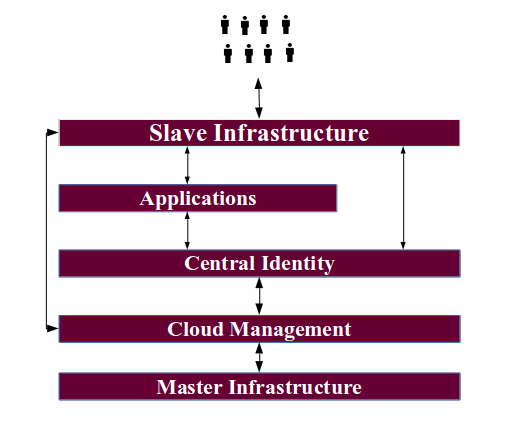
\includegraphics[height=8cm]{./idea.png} \\
%% \caption{Archtitecture\label{fig:idea}} 
%%\end{figure}
%
%\begin{figure}[H]
% 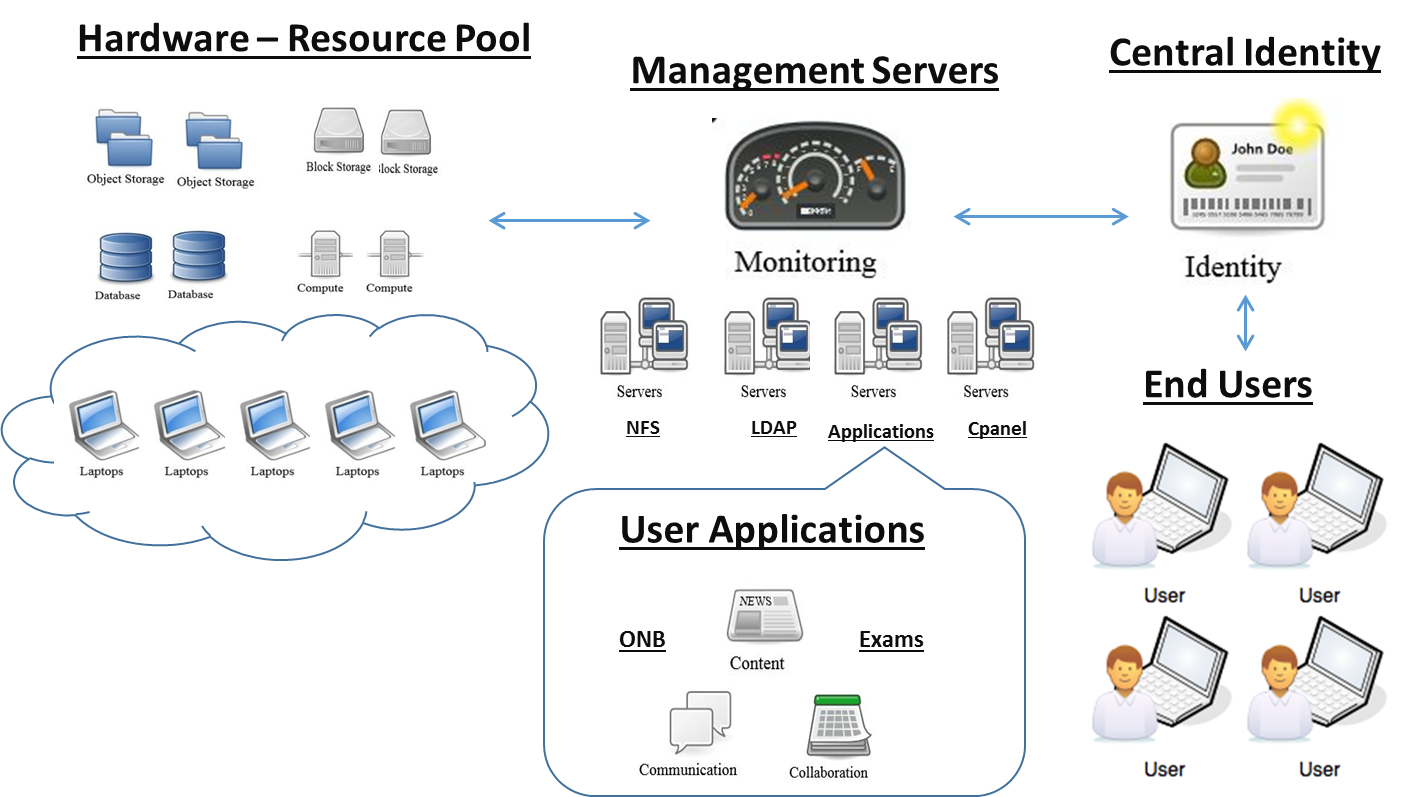
\includegraphics[height=8cm]{./all.png} \\
% \caption{Archtitecture Implementation\label{fig:all}} 
%\end{figure}
%
%\end{center}
%
%\pagebreak
%
%\section{Architecture Explained }
%
%\subsection{Central Identity}
%\hspace{1cm} It is an Identity as a Services for network based applications and web services using API calls. Using this we are going to implement the services like single sign-on, role based user identity thus reduces the redundancy of data.
%
%\begin{center}
%
%\begin{figure}[H]
% 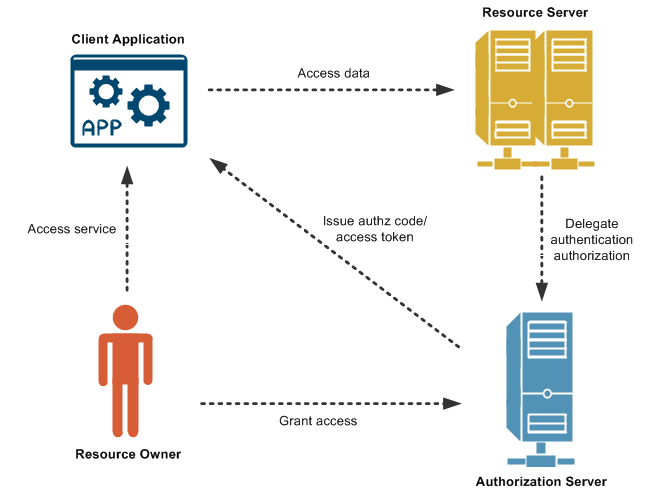
\includegraphics[height=8cm]{./oauth.png} \\
% \caption{Central Identity\label{fig:oauth}} 
%\end{figure}
%
%\end{center}
%
%\subsection{Hardware Resource Pool}
%
%\hspace{1cm} Here we will try to cluster all the hardware resources provided as a pool, by this we can achieve highly configurable systems
%
%
%\begin{figure}[H]
% 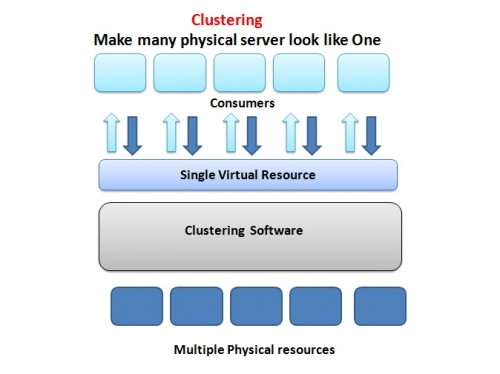
\includegraphics[height=6cm]{./cluster.jpg} \\
% \caption{Hardware Resource Pool \label{fig:cluster}} 
%\end{figure}
%
%
%
%
%\section{Advantages}
%
%\begin{itemize}
%	\item Well structured \& controllable Network Administraion
%	\item Efficient hardware utilization
%	\item No registration for new Network based applications through Central Identity API
%	\item Provding Virtual Machines with high hardware configuration for Researchers \& Developers
%	\item Facilitates high availability of all web-services (Like ONB, Examination, Course registration Helping hand website, SDCAC website and all departmental websites etc.)
%	\item It will provide High computational power for research work of Faculty, research scholars and students.
%	\item Get full recovery and  achieve 100\% Services up time.
%\end{itemize}
%\pagebreak
%
%\section{Requirements}
%\begin{center}
%\begin{itemize}
%\item  10 Laptops with 2 NICs
%\begin{itemize}
%	\item  8 GB RAM systems - 4 
%	\item  4 GB RAM systems - 6 
%	\begin{itemize}
%		\item (2013 Sep Model (Acer Travel mate) available with 4 GB Ram, 500 GB HD and One NIC. We need to extend 4GB Ram to 8 GB RAM, We need to Extend One more NIC)
%	\end{itemize}
%	
%\end{itemize}
% 
%\item Internet Facility 
%\begin{itemize}
%	\item 10 Static IP with Full Internet Access For Laboratory [ SF6 – 10.4.16.x]
%	\item 2 Proxy Accounts with Unlimited Downloading 
%	\item Uninterrupted Internet Connectivity with 512KBPS+ Downloading Speed.
%	\item Basically we getting 10-15 KB Speed while Class Hours. This thing should be avoided.
%\end{itemize}
%
%\item Uninterrupted Power Supply For Laptops in Lab
%\item 24 x 7 Lab availability
%\item Configurable 24 Port switches’ for construction private network with in Cloud Laboratory. 
%\end{itemize}
%\end{center}

\end{document}